\documentclass[11pt]{book}
\usepackage[utf8]{inputenc}
\usepackage[IL2]{fontenc}
%\usepackage[czech]{babel}
\usepackage[]{graphicx}
\usepackage{caption}
\usepackage{subcaption}
\usepackage{indentfirst}
\usepackage{algorithm}
\usepackage[noend]{algpseudocode}
\usepackage{float}
\usepackage{enumitem}
\usepackage{amsmath}

\newcommand{\N}{\mathbb{N}}
\newcommand{\R}{\mathbb{R}}
\newcommand{\Q}{\mathbb{Q}}
\newcommand{\Z}{\mathbb{Z}}
\newcommand{\E}{\mathbb{E}}
\newcommand{\BigO}{\mathcal{O}}

\DeclareMathOperator*{\argmax}{arg\,max}
\DeclareMathOperator*{\argmin}{arg\,min}

\makeatletter
\def\BState{\State\hskip-\ALG@thistlm}
\makeatother

\usepackage{amsmath,amsfonts,amssymb}
\usepackage{a4wide}
\usepackage{hyperref}
\usepackage{float}

\usepackage{filecontents}
\begin{filecontents*}{trial.bib}
@article{projectionFeasibility,
	author = {Ion Necoara, Peter Richtárik, Andrei Patrascu},
	title = {Randomized projection methods for convex feasibility},
	note = "\url{http://141.85.225.150/papers/feasibility.pdf}",
	year = {2017}
}
@article{iterativeLinearSystems,
	author = {Robert Mansel Gower, Peter Richtárik},
	title = {Randomized Iterative Methods for Linear Systems},
	journaltitle = {SIAM Journal on Matrix Analysis and Applications},
	note = "\url{http://epubs.siam.org/doi/abs/10.1137/15M1025487}",
	year = {2015}
}
@thesis{sketchAndProject,
	author = {Robert Mansel Gower},
	title = {Sketch and Project: Randomized Iterative Methods for Linear Systems and Inverting Matrices},
	institution = {The University of Edinbourgh},
	note = "\url{www.arxiv.org/pdf/1612.06013.pdf}",
	year = {2016}
}
@online{GD,
	author = {RadhaKrishna Ganti},
	title = {Convergence rate of gradient descent algorithm},
	note = "\url{www.rkganti.wordpress.com/2015/08/21/convergence-rate-of-gradient-descent-algorithm/}",
	year = {2015}
}
@article{SGD,
	author = {Simon Lacoste-Julien, Mark Schmidt, and Francis Bach},
	title = {A simpler approach to obtaining an $\mathcal{O}(1/t)$ convergence rate	for the projected stochastic subgradient method},
	note = "\url{www.arxiv.org/pdf/1212.2002v2.pdf}",
	year = {2012}
}
@article{SAGA,
	author = {Aaron Defazio, Francis Bach},
	title = {SAGA: A Fast Incremental Gradient Method With Support for Non-Strongly Convex Composite Objectives},
	note = "\url{www.di.ens.fr/~fbach/Defazio_NIPS2014.pdf}",
	year = {2014}
}
@article{kaczmarz,
	author = {Thomas Strohmer, Roman Vershynin},
	title = { randomized Kaczmarz algorithm with exponential convergence},
	note = "\url{www.arxiv.org/pdf/math/0702226.pdf}",
	year = {2007}
}
@article{acceleration,
	author = {Aleksandar Botev, Guy Lever, David Barber},
	title = {Nesterov’s Accelerated Gradient and Momentum as approximations to Regularised Update Descent},
	note = "\url{www.arxiv.org/pdf/1607.01981.pdf}",
	year = {2016}
}
@article{kosto,
	author = {konstantin},
	title = {?},
	note = "\url{?}",
	year = {2018?}
}
\end{filecontents*}

\begin{document}
\title{\textbf{TODO rename}}
\author{Slavomír Hanzely}
\maketitle

\chapter*{\centering Abstract}
\addcontentsline{toc}{chapter}{Abstract}

This project is about constraint optimization. It is focused on sketching algorithm finding point close to closed convex set by projecting on supersets and also on SAGA algorithm. Both algorithm have been described with motivation behind them. Their optimal parameters have been tested and compared with experimentally best parameters. It was shown, that theoretical parameters are not best in practice, however they are not much worse than experimentally best ones. They might be used in practice, because it is hard to compute experimentally better ones.

\tableofcontents

\chapter{Introduction}

In this work, we are working with complicated convex set $X$ defined as intersection of large number of simple constraints. Starting with convex feasibility problem, our goal is to quickly find point close to the convex set. Exact computation may be done, but if $X$ is complicated, it may be lengthy or infeasible. Thus direct computation is to be avoided.

The type of indirect algorithms, that could be used for this kind of problem, are iterative ones. Starting with initial guess, which point could be in the set, they are iteratively improving their guess, until they are sufficiently close. They use to find point near optimum much faster than exact computation.

In our case, we are having a large number of simple constraints. Working with all of them in each step is slow. Hence, we are interested in algorithms, that work with only part of all constraints in each step - so called stochastic algorithms. Stochastic algorithms use to involve randomness and as measure of convergence speed, expected distance from optimum is used.

In this work, convex feasibility problem is solved by sketching algorithm, which in each step project current point on randomly chosen individual constraint.\\

Convex feasibility problem could be equivalently reformulated in many ways, so that the set of solutions reminds the same. One of the options is to reformulate it as stochastic optimization problem with specific distribution of points. Natural choice of algorithm for this newly constructed problem is well-known gradient descent. It turns out that stochastic gradient descent on this reformulated problem does the same as sketching algorithm on original problem.\\

In both of the original and reformulated problem, we were looking for arbitrary point sufficiently close to set $X$. If points in $X$ are not equally good for us, we need to do something different. We may assign values to points (using some function) and then minimize that function. Let's suppose, that we want to find point in $X$, that also minimizes function, defined as sum of simple functions.

Our new problem turned out to be stochastic minimization problem over set $X$. We could once more reformulated it as stochastic optimization problem without constraints (its goal is to minimize sum of large number of functions) and try to use iterative algorithms on it. As mentioned, large number of functions make non-stochastic gradient descent infeasible.

One of the possible approaches is to use classical stochastic gradient descent. It is necessary to remind, that stochastic gradient descent is moving according to subgradients, which are nonzero even in optimum. Thus stochastic gradient descent does not stop at optimum unless the size of steps is being reduced to zero. However, reducing size of steps leads to slower convergence rate.

Second option, how to make stochastic modification of gradient descent that will stop at optimum without reducing size of the steps, is to move according to gradient of sum (or average) of all functions in each step and make this gradient to go to $0$. If algorithm find point, that the function has average gradient $0$  in it, than that point is minimum (local or global).

For this kind of approach, it is possible to use SAGA algorithm. It has saved all (probably outdated) gradients in Jacobian and their average. In each step, it updates one gradient, their average and then does gradient descent step (using average of all gradients). SAGA algorithm is stochastic, in each step it only compute gradient of one function. It could be shown, that this algorithm converges as fast as gradient descent (thus faster than stochastic gradient descent).\\

In each iteration of SAGA, one column of Jacobian is updated and rest of Jacobian stays the same. We could take updating of Jacobian as using sketching algorithm again and projecting old Jacobian to superset of new Jacobian (changing only one column). Thus we got by circle to algorithm, which we had been beginning with.\\

The goal of this work is to intuitively present motivation behind both sketching and SAGA algorithms, test them in practice and find out, whether there is possibility to improve theoretical best parameters. For both sketching and SAGA algorithms, there are also included experimental testing of their performance and also comparison, how fast does they converge with different parameters. Project was implemented in the language Julia, that is very fast and simple to use, especially for matrix operations.

\chapter{Convex feasibility}

\section{Problem definition}

Convex feasibility problem is defined as following: Given nonempty closed convex set $X$, find a point $x \in X.$\\

It is possible to compute point $x$ as projection on $X$. However, exact computation could be hard if the dimension of $X$ is high or in general, if $X$ is a complicated set. In many cases, it is sufficient to find a point close to $X$. If we can do it fast, a lengthy or infeasible computation can be avoided.\\

Suppose we have given $X_2 , X_2 , \cdots X_n$ - supersets of $X$, which are simple and easy to project on them. If we cannot compute point in $X$ directly, we could try to take point $x_0$ in space and try to move it iteratively to solution. To get closer to solution, we could use supersets of $X$. If we look at projection of $x_0$ on superset $X_j$, it is not further to solution than $x$. So we have found point closer to intersection than $x_0$.

In each step we could iteratively get $x_{i+1}$ as projection of $x_i$ on $X_j$ (for randomly chosen $j$) and we get points closer and closer to intersection of supersets.

Under some technical assumptions on those supersets, it can be proved that by successive projecting on random $X_i$ we can get very quickly (depending on the condition number of the problem) close to $X$ with arbitrary probability. Let $\Pi(x, Y)$ be projection of point $x$ on the convex set $Y$, $$\Pi(x,Y) = \min_{y \in Y} ||x-y||.$$ The algorithm for approximating the point from $X$ (stochastic) is following:

\begin{algorithm}[H]
	\caption{Set sketching \cite{projectionFeasibility}\cite{kaczmarz}}
	\label{alg:set sketch}
	\begin{algorithmic}[1]
		\State Choose parameters $\omega, \tau$ and $ X_i$
		\State Choose initial point $x_0$
		\For{$k = 0, 1, 2 \cdots$}:
		\State $x_{k+1} \leftarrow (1 - \omega)x_k + \frac{\omega}{\tau}\sum_{i \in S_k} \Pi(x_k, X_i )$
		\EndFor
	\end{algorithmic}
\end{algorithm}

\noindent
where $S_k$ is a random subset of $\{ 1, \dots , n\}$ for every $k$, $|S_k|=\tau$ ($S$ samples supersets $X_i$).\\

Parameter $\omega$ specifies the size of the step, parameter $\tau$ determines a number of the sets to project on every iteration.\\

As mentioned above, it can be shown that the algorithm converges relatively quickly even though $X$ is a complicated set often given by a very large amount of data. To get to distance $d$ from optimum, it is needed $\mathcal{O} (log(\frac{1}{d}))$ iterations\cite{sketchAndProject}\cite{kaczmarz}.  However, the optimal parameter selection for the algorithm is unclear. Since this area is not sufficiently examined, the theory is built only for the case where the length of step $\omega$ is constant.\\

\section{Implementation}

In simulation, convex set is represented by set of $x$ such as $Ax=b$ (for randomly generated matrix $A$ and vector $b$) intersected with unit ball.

Variant with only linear system is easy, and already known as random Kaczmarz method \cite{kaczmarz} \cite{iterativeLinearSystems}. We are interested in case, where there are also other convex sets. As convex sets to be projected on, I have chosen the affine subspaces (rows of matrix $A$) and the ball with center at origin.

Simulation took place in $\R^{10}$.\\

During the simulation, program computed (for each processed $x_k$) distance from the real projection spot (later I'll call it just distances). Also for processed $x_k$ it computes, for which $\omega$ would be the new point closest to the real projection spot. It is the best $\omega$, that could be chosen for given (concrete) $x_k$ (later, I'll call it just best omegas).

As the output of the simulation, these two informations (distances and best omegas) were plotted. Because the distances of the points $x_k$ from the real projection spot are exponentially decreasing, plotted graph has axis $y$ with logarithmic scale.\\

The most relevant data to compare speed of convergence is known convergence rate of only linear system (excluding ball). In $k$-th iteration, its expected distance from optimum is $||x-x_0||(1-\lambda_{min})^k$ \cite{kaczmarz}, where $\lambda_{min}$ is smallest nonzero eigenvalue of $A^TA$ (this exponential function I'll call theoretical convergence). So by adding projections on ball it should still be good approximation.

As baseline, theoretical convergence was plotted (it is also exponential function).

\section{Simulation setup}

There were multiple simulation setups, they differed in following parameters:

\begin{list}{•}{}
	\item $\tau$, that is chosen from set $\{ 1, 3, 8 \}$.
	\item Whether unit ball is between $X_i$ or it is excluded.
	\item $\omega$, whether it is constant\footnote{As constant, it was chosen 1} for whole simulation or it chosen each step for optimal value.
\end{list}

For each combination of parameters above, multiple simulation were run (and graphs saved). Below, there are some of the graphs, for each combination of parameters one.\\

\newpage
\textbf{Description of graphs}:
\begin{itemize}[noitemsep]
	\item X axis shows iteration
	\item Y axis shows distance (logarithmic scale)
	\item Theoretical convergence is orange line.
	\item Distance from projection is blue line.
	\item Best omega, that could be chosen (for every concrete $x_k$) is drawn as grey dot (for $x_k$).
\end{itemize}

\begin{figure}[H]
	\centering
	\begin{subfigure}{.5\textwidth}
		\centering
		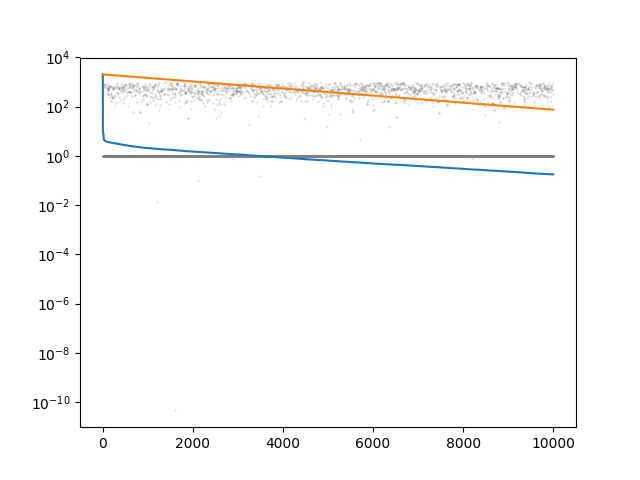
\includegraphics[width=.8\linewidth]{f1b.png}
		\caption{fixed $\omega$}
		\label{fig:sub1}
	\end{subfigure}%
	\begin{subfigure}{.5\textwidth}
		\centering
		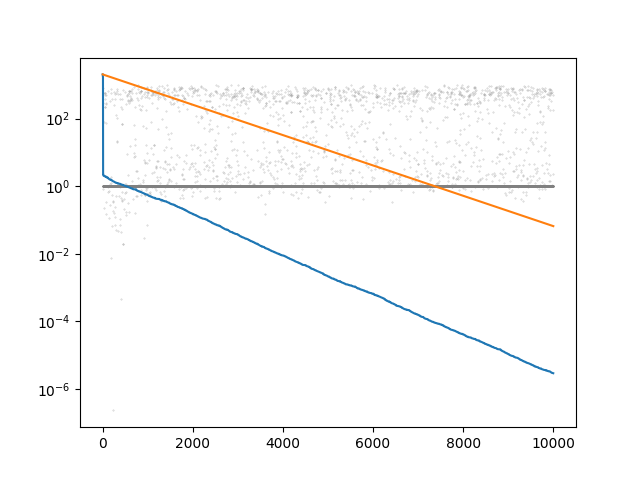
\includegraphics[width=.8\linewidth]{b1b.png}
		\caption{best omega}
		\label{fig:sub2}
	\end{subfigure}
	\caption{$\tau=1$, with ball}
	\label{fig:test1}
	
	\centering
	\begin{subfigure}{.5\textwidth}
		\centering
		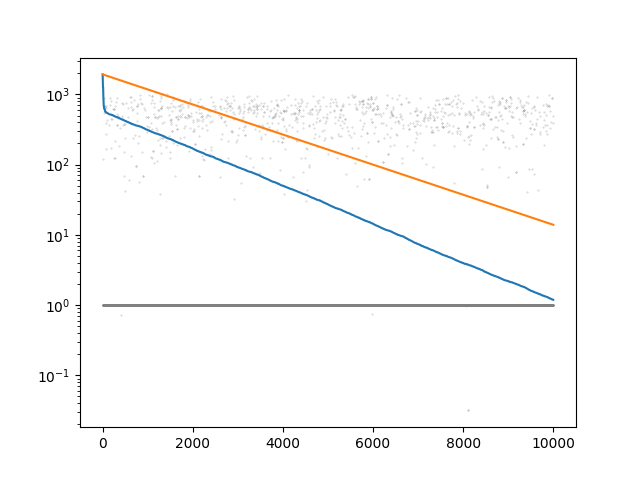
\includegraphics[width=.8\linewidth]{f1n.png}
		\caption{fixed $\omega$}
		\label{fig:sub3}
	\end{subfigure}%
	\begin{subfigure}{.5\textwidth}
		\centering
		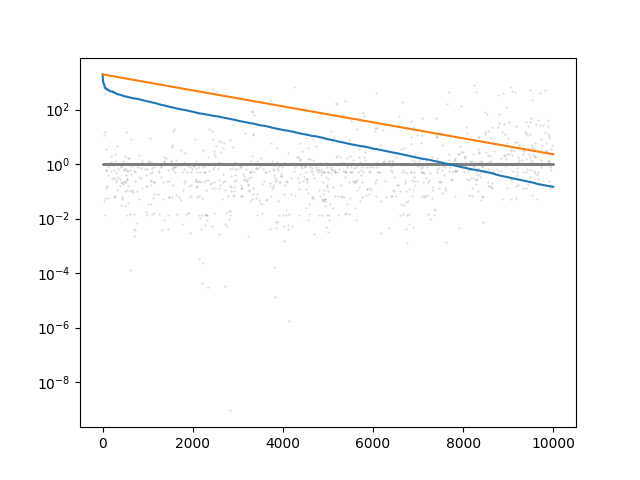
\includegraphics[width=.8\linewidth]{b1n.png}
		\caption{best omega}
		\label{fig:sub4}
	\end{subfigure}
	\caption{$\tau=1$, without ball}
	\label{fig:test2}
	
	\centering
	\begin{subfigure}{.5\textwidth}
		\centering
		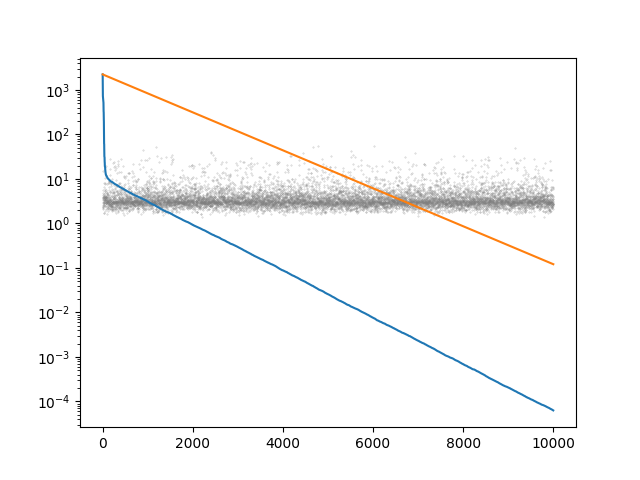
\includegraphics[width=.8\linewidth]{f3b.png}
		\caption{fixed $\omega$}
		\label{fig:sub5}
	\end{subfigure}%
	\begin{subfigure}{.5\textwidth}
		\centering
		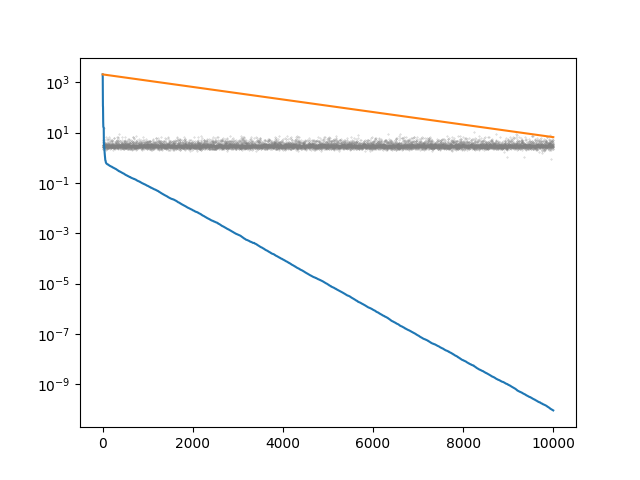
\includegraphics[width=.8\linewidth]{b3b.png}
		\caption{best omega}
		\label{fig:sub6}
	\end{subfigure}
	\caption{$\tau=3$, with ball}
	\label{fig:test3}
\end{figure}

\begin{figure}[H]
	\centering
	\begin{subfigure}{.5\textwidth}
		\centering
		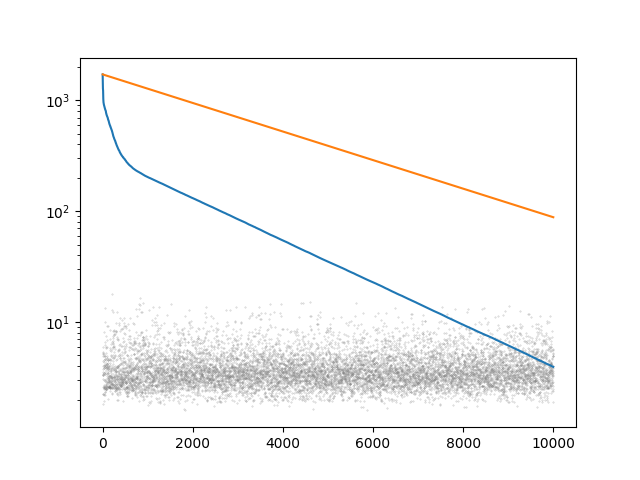
\includegraphics[width=.8\linewidth]{f3n.png}
		\caption{fixed $\omega$}
		\label{fig:sub7}
	\end{subfigure}%
	\begin{subfigure}{.5\textwidth}
		\centering
		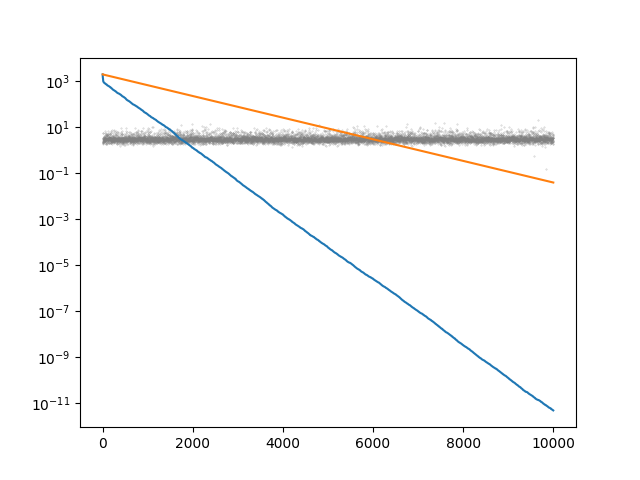
\includegraphics[width=.8\linewidth]{b3n.png}
		\caption{best omega}
		\label{fig:sub8}
	\end{subfigure}
	\caption{$\tau=3$, without ball}
	\label{fig:test4}
	
	\centering
	\begin{subfigure}{.5\textwidth}
		\centering
		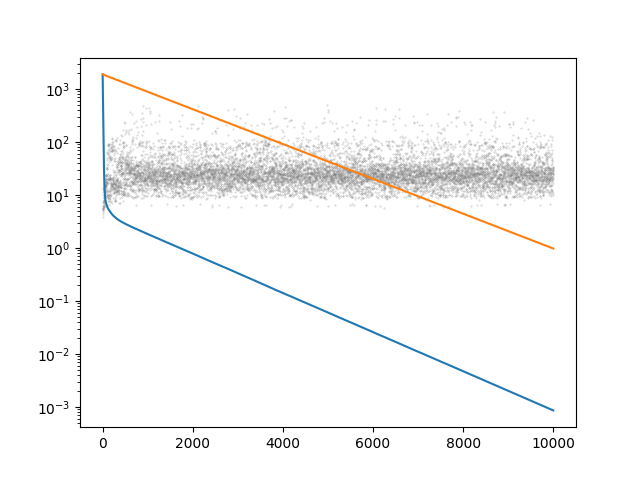
\includegraphics[width=.8\linewidth]{f8b.png}
		\caption{fixed $\omega$}
		\label{fig:sub9}
	\end{subfigure}%
	\begin{subfigure}{.5\textwidth}
		\centering
		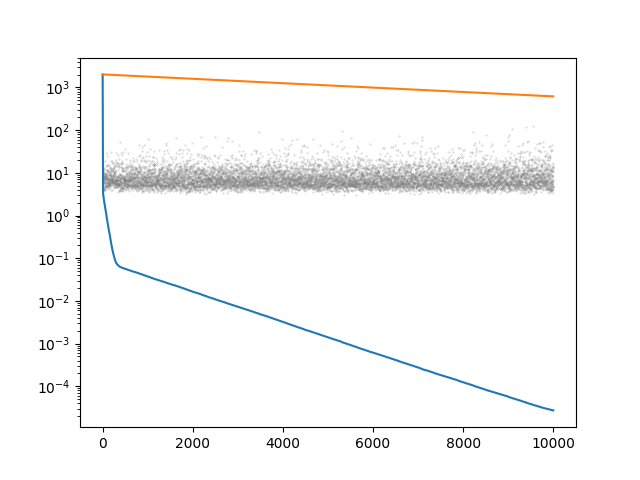
\includegraphics[width=.8\linewidth]{b8b.png}
		\caption{best omega}
		\label{fig:sub10}
	\end{subfigure}
	\caption{$\tau=8$, with ball}
	\label{fig:test5}
	
	\centering
	\begin{subfigure}{.5\textwidth}
		\centering
		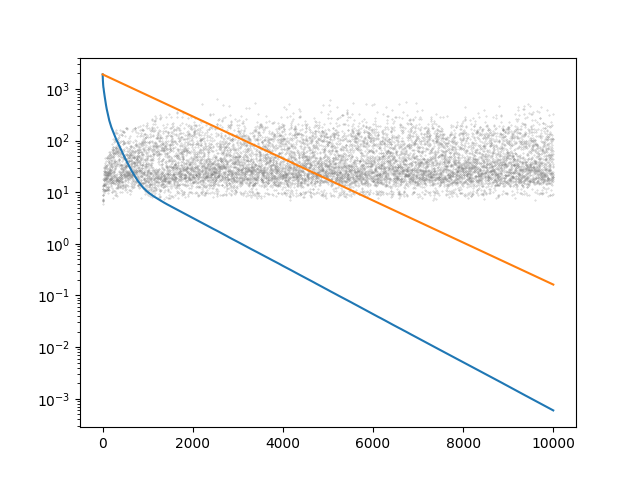
\includegraphics[width=.8\linewidth]{f8n.png}
		\caption{fixed $\omega$}
		\label{fig:sub11}
	\end{subfigure}%
	\begin{subfigure}{.5\textwidth}
		\centering
		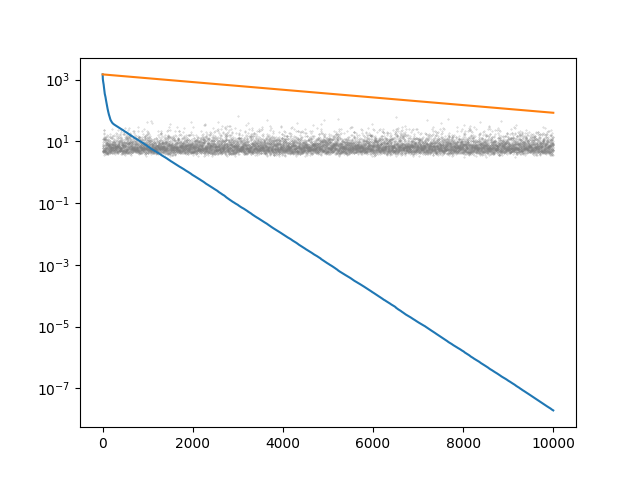
\includegraphics[width=.8\linewidth]{b8n.png}
		\caption{best omega}
		\label{fig:sub12}
	\end{subfigure}
	\caption{$\tau=8$, without ball}
	\label{fig:test6}
\end{figure}

\newpage

\section{Simulation result}

Algorithm was successfully implemented and simulated, plenty of graphs were drawn here.\\

In every setup, distances of points $x_k$ in graph made line (from some point), thus distances were always decreasing exponentially.\\

For $\tau=1$, we were projecting only on 1 line (or ball) each iteration. This setup computed iterations fastest, but the rate of converging was slowest. There was no visible difference between setting $\omega$ as constant 1 or choosing best omega each in every iteration. It was caused by fact, that for $\tau=1$ were values of best omegas around $1$ (that was also fixed value of $\omega$).\\

With increasing $\tau$ (for fixed $\omega$), simulation was converging a bit faster with each iteration (lines of graphs were steeper), but computation of one iteration was slower (because it is necessary to compute $\tau$ projections each iteration).

Changing fixed $\omega$ for best omega lead to huge convergence speedup. Distances of $x_k$ curve was much steeper than theoretical convergence. However, in the simulation, best omegas were computed from the real projection point, thus it is not possible to use them for convergence speedup in practice.\\

Setups with projecting on a ball in beginning of the simulation jumped into smaller distance, but after that, the converge rate was same (even a bit slower) as setup without projection on ball (with same $\tau$ and $\omega$). It is caused by the fact, that projecting on ball from outside of the ball lead to big distance reduction. Once point is inside in the ball, projecting on the ball makes no difference.

Simulation showed, that current estimation of $\omega$ is not the best estimation in practice. Thus it might be possible to prove better estimation.

\section{Changing set of solution in convex feasibility problem}

In our setup, we were interested in $X$ to be set of solutions of linear system $Ax=b$ intersected with unit ball.

We could also set $X$ to be set of solutions $x$ such as $Ax=I$, by solving convex feasibility problem we will finding inversion of matrix $A$.

We may also set $X$ to be set of solutions $x$ such as $x=B$, for fixed matrix $B$. This problem is trivial, but it can also be solved using sketching. It converges to distance $d$ in $log(\frac{n}{d(n-1)})$\label{xIsB} iterations, where $n$ is dimension of $x$.\\

\section{Alternative angles of views on convex feasibility problem}
As mentioned in introduction, convex feasibility problem could be equivalently reformulated in many ways, so that the set of solutions reminds the same. Here are few different angles of view.

Convex feasibility problem can be viewed as minimization problem over set $X$, find $$\argmin_{x \in X} 0.$$

It may also be reformulated as stochastic optimization problem \cite{sketchAndProject}: $$\text{minimize } f(x)=\E_{S \sim D}[f_S(x)],$$ where $$f_S(x) = \frac{1}{2}||x-\Pi_{x_S}(x)||^2.$$
Stochastic gradient descent on latter problem does the same as sketching algorithm on original problem.\\

We have got algorithm, that can find some point in convex set. However, it can find arbitrary point near to set $X$. If points in $X$ are not equally good for us, we need to do something different. We may assign values to points (using some function) and then minimize that function. Let's suppose, that we want to find point in $X$, that also minimizes sum of large number of simple functions over $X$, we would like to find $$\argmin_{x \in X} F(x),$$ where $F(x)=\sum_{i=1}^{l}f_i(x).$



\chapter{Optimization with many constraints}

\section{Problem definition}
Problem is defined as following: Given a large set of functions $f_1,f_2,\cdots,f_l$ (for $f_i: \R^n \rightarrow \R$) and complicated set of constrains $X = \cap_{j=1}^m X_j$ (for simple convex constraints $X_j$), find a point $x \in \R^n$ that satisfies $X$ and minimize average of functions at $x$: $$ \min_{x \in \R^n \cap X} \frac{1}{l}\sum_{i=1}^l f_i(x).$$

Lets denote $F(x)=\frac{1}{l}\sum_{i=1}^l f_i(x)$, the problem is to minimize $F(x)$ also satisfying given constraints.\\

Instead solving that problem, we will solve following problem: \label{solvedProblem}
$$ \min_{x \in \R^n} \frac{1}{l}\sum_{i=1}^l f_i(x) + \lambda h(x),$$
where $h(x)=\frac{1}{2m}\sum_{j=1}^m ||x-\Pi_{X_j}(x)||^2$.

Our new problem is optimization problem without constraints.
Optimal solutions of original problem are also optimal solutions of new problem (when $x \in X$, then $||x-\Pi_{X_j}(x)||=0$ for each $X_j$, thus $h(x)$ is zero).

It could be shown, that solution of new problem is approximate solution of previous problem, accuracy of approximation depends on parameter $\lambda$ (the bigger $\lambda$, more accurate solution). Thus minimization problem with constraints is reduced to minimization problem without constraints, if we assume convexity of functions $f_i$ and $h$, we could find solution using gradient descent:\\

\begin{algorithm}[H]
	\caption{Gradient descent}
	\label{alg:gd}
	\begin{algorithmic}[1]
		\State Choose parameter $\alpha$
		\State Choose initial point $x_0$
		\For {$k = 0, 1, 2, \cdots$}
		\State $x_{k+1} \leftarrow x_k - \alpha\nabla F(x_k) $
		\EndFor
	\end{algorithmic}
\end{algorithm}

Gradient descent is much faster than exact computation, on strongly convex functions it converges to distance $d$ with $\mathcal{O}(log(\frac{1}{d}))$ iterations \cite{GD} . This convergence rate is referred as linear. However, it is not appropriate for this problem. In our case, both the number of functions $f_i$ and number of constraints $X_i$ are large, so it may not be able to process all data at once.

Hence it is necessary to use stochastic version. Let's denote $\tau$ minibatch size (number of functions processed in one step), let's define $\nabla F_k(x_k)$ as following: $$\nabla F_k(x_k) = \frac{1}{\tau}\sum_1^\tau \nabla f_{s_1}(x_k)$$ where $\{s_1, s_2, \cdots, s_\tau\}$ is subset of $\{1,2,\cdots, l \}$. $\nabla F_k(x_k)$ is average gradient of randomly chosen $\tau$ functions at point $x_k$. Stochastic gradient descent is following:

\begin{algorithm}[H]
	\caption{Stochastic gradient descent}
	\label{alg:sgd}
	\begin{algorithmic}[1]
		\State Choose parameters $\alpha_0$, $\alpha_1$, $\dots$.
		\State Choose initial point $x_0$
		\For {$k = 0, 1, 2, \cdots$}
		\State $x_{k+1} \leftarrow x_k - \alpha_k\nabla F_k(x_k) $
		\EndFor
	\end{algorithmic}
\end{algorithm}

For stochastic gradient descent to stop at optimum, it is necessary for parameters $\alpha_k$ to satisfy: $\lim_{k \rightarrow \infty}\alpha_k=0 $. Convergence rate of stochastic gradient descent is slower than gradient descents rate, it converges to distance $d$ with $\mathcal{O}(\frac{1}{d})$ iterations \cite{SGD}. This convergence rate is referred as sub-linear.\\

We would like to use algorithm that does not compute all gradients at each step (like stochastic gradient descent), but stops at optimum without decreasing stepsize parameter $\alpha$ (like gradient descent).\\

Our algorithm is called SAGA, it will move according to average gradient of functions, but it will not compute average gradient exactly. It will store list of (probably outdated) gradients of functions and their average. In each step, it updates $\tau$ gradients (randomly chosen), it updates average of all gradients and does step of gradient descent.\\

The state of the algorithm is represented by current point $x_k$, current estimate of gradients of all functions $f_i$ and all addends of sum $h$ (that have form $||x-\Pi_{X_i}(x)||^2$) (in Jacobian $J$) and average of gradients $$\nabla F_{avr}= \frac{1}{l+m}\left( \sum_{i=1}^l \nabla f_i + \lambda\sum_{i=1}^m \nabla ||x-\Pi_{X_i}(x)||^2 \right).$$ In each step current point $x$ is used for better estimation of Jacobian and then current estimation of jacobian is used for step in gradient descent.\\

This algorithm requires functions $f_i$ and all addends of sum $h$ ($||x-\Pi_{X_i}(x)||^2$) to be $\mu$-strongly convex and Lipschitz smooth with constant $L$. Former means, that for $\mu>0$ for all x, y holds $$\langle \nabla f(x) - \nabla f(y), (x-y) \rangle \geq \mu ||x-y||_2^2. $$
Later means, that exists constant $L$, that for all x, y holds $$||\nabla f(x) - \nabla f(y)||_2 \leq L ||x-y||_2.$$ Both constants $\mu$ and $L$ bound, how much function values $\nabla f(x)$ could change much when moving $x$.

\begin{algorithm}[H]
	\caption{SAGA \cite{SAGA}}
	\label{alg:saga}
	\begin{algorithmic}[1]
		\State Choose parameters $\alpha$, $\tau$, $r$, $s$.
		\State Choose initial point $x_0$, and initial Jacobian $J$ of functions $f_1$, $f_2$, $\cdots$, $f_l$.
		\State Compute initial mean of functions $f_i$.
		\For {$k = 0, 1, 2, \cdots$}
		\State choose $\tau$ functions (uniformly randomly)
		\State update gradient of each the function, also average of gradients
		\State do gradient descent step $\quad x_{k+1} \leftarrow x_k - \alpha\nabla F_{avr}(x_k) \quad$
		\EndFor
	\end{algorithmic}
\end{algorithm}

\textbf{Remark:} SAGA algorithm with $\tau=l+m$ is gradient descent algorithm.\\

Convergence rate of SAGA is referred as linear, it converges to distance $d$ with $\mathcal{O}(log(\frac{1}{d}))$ iterations \cite{SAGA}, it should as fast as gradient descent.\\

\begin{figure}[H]
	\centering
	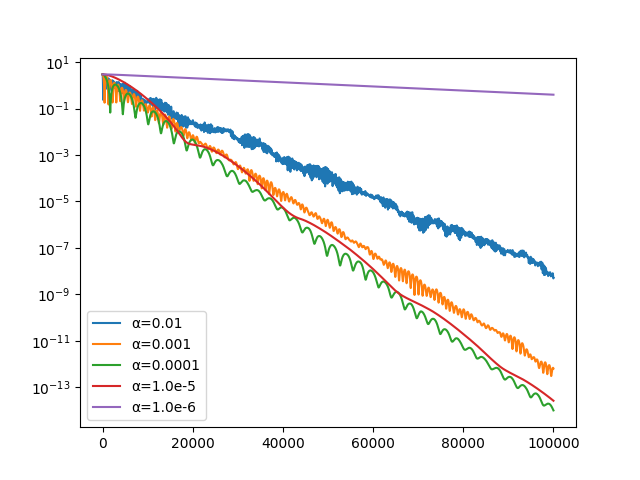
\includegraphics[width=0.7\linewidth]{saga_convergence.png}
	\caption{convergence of SAGA algorithm for different stepsize $\alpha$}
	\label{fig:saga}
\end{figure}

\section{Parameters in theory}

First of all, let's take a look on parameter $\lambda$ in $F(x)+\lambda h(x)$ (function, we want to minimize). As mentioned above, bigger $\lambda$ put more emphasis on constraints. However, bigger $\lambda$ increase the conditional number of that function, so overall convergence speed is slower.\\

The most import parameter in our simulation is minibatch parameter $\tau$. The bigger minibatch parameter $\tau$, the more functions are updated each step. Consequently, the average gradient of functions is more precise, so $x_i$ will go more faster to optimum. Also for bigger $\tau$ the optimal stepsize parameter $\alpha$ may be bigger. Hence the algorithm should converge in less iterations. But the bigger minibatch parameter $\tau$ leads to more gradients computation in each step, so the iterations are slower to compute.

It is not clear, what combination of parameters $\tau$ and $\alpha$ leads to fastest convergence. As measure of speed of convergence, number of gradients computed before convergence was used. In theory, algorithm should be fastest when $\tau=1$, and with increasing $\tau$, it should get monotonically worse, the worst possible result is for $\tau = k+m$ (gradient descent case).

Let's denote $L$ Lipschitz smooth constant for every $f_i$ and $\mu$ strongly convex constant for every $f_i$. Fastest convergence for strongly convex functions is achieved for $\alpha = \frac{1}{2(\mu n + L)}$. For non-strongly convex functions, the best convergence rate is achieved for $\alpha = \frac{1}{3L}$. These values are best for general functions, so it may be possible that they are not optimal in practice. In simulation we would like to find out, how good is best stepsize parameter in practice and how does it change with increase of minibatch size.


\section{Implementation}

The simulation took place in $\R^{10}$, number of functions was $1500$, number of constraints was $500$.\\

Functions $f_i$ were chosen as quadratic functions, $f_i(x) = (A_ix-b_i)^T(A_ix-b_i)$, for random matrix $A_i$ (of size $10 \times 10$) and random vector $b_i$ (of size $10$). Constraints were chosen to be linear, they were given by rows of matrix $A_cx=b_c$, for random matrix $A_c$ (of size $500 \times 10$), and random vector $b_c$ (of size $10$).\\

In our setup, $L$ is the biggest eigenvalue of functions $f_i$ and $\mu=0$.

\section{Simulation setup}

If stepsize parameter was fixed for different minibatch sizes, the plots looked like following:

\begin{figure}[H]
	\centering
	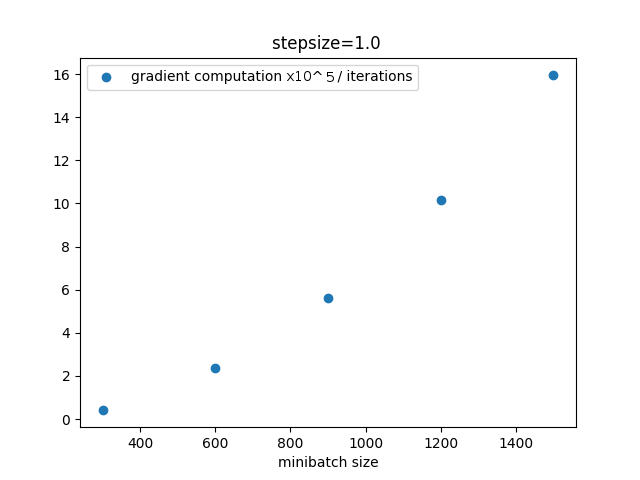
\includegraphics[width=.7\linewidth]{fixed_stepsize.png}
	\caption{fixed stepsize for all minibatch sizes}
	\label{fig:fixed stepsize}
\end{figure}

It turned out, that optimal stepsize parameters for different minibatch sizes were completely different. Increase of gradient computation in Figure \ref{fig:fixed stepsize} was caused by wrong stepsize parameter choice. Hence it is necessary to compute experimentally optimal stepsize parameter for each minibatch size.\\


In each simulation, functions, initial point $x_0$ and parameters $\tau, \lambda$ were fixed. Then different minibatch sizes $\tau$ were chosen. For each of them experimentally best parameter $\alpha_{\tau_i}$ was found and number of gradient computed until convergence (for $\alpha_{\tau_i}$) was plotted. 

To find $\alpha_{\tau_i}$, many different values were tried, the best of them was picked. Initial guesses had form $10^t$ (to capture $\alpha$ with low relative error to optimal value), after observation, more values were tried close to the best guess so far.\\

\section{Simulation result}

\begin{figure}[H]
	\centering
	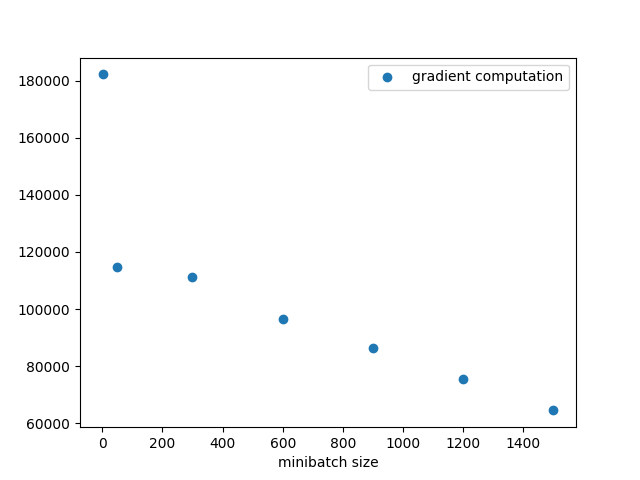
\includegraphics[width=.7\linewidth]{optimal_stepsize.png}
	\caption{experimentally optimal stepsize}
	\label{fig:optimal stepsize}
\end{figure}



For minibatch size $\tau=1$ was experimentally optimal stepsize parameter $\alpha$ much smaller than theoretical optimal parameter. Choosing $\alpha$ to be theoretical best one lead to much slower convergence speed.

With increasing $\tau$ number of gradient computation necessary to converge decreased, difference was $10\% - 66\%$ decrease of gradient computation.

Ratio between gradient computation with theoretical and experimental stepsizes increased with increase in $\lambda$. For $\lambda <1$, ratio was less than $20\%$, for $\lambda=100$, it was $\sim 60\%$, for $\lambda=1000$, it was even more than $95\%$. It may be caused by uniform function sampling.\\

In this setup theoretical value of $\alpha$ for $\tau$ lead to slower convergence rate. However, computing experimentally better parameters required much more computation than converging with theoretical parameters, thus in practice, it would be faster to use theoretical parameters.

\chapter{Conclusion}

\section{Jacobian sketching}

Let's look once again on sketching algorithm. We had convex set $X$ as set of solutions $x$ in $Ax=b$. In each step, we were projecting point $x_k$ on superset of $X$, that had form of rows of matrix $A$.

Later, in SAGA algorithm, we have been updating columns of Jacobian in each iteration. This update could be viewed as projecting old Jacobian to column of new Jacobian. It change only one column at time. This is exactly convex feasibility problem, that what we were doing before.

We could take updating of Jacobian as convex feasibility sketching achieved by projecting old Jacobian to supersets (columns) of new Jacobian, we would like to find $x \in X$, where $X=Jacobian_{real}$. It is similar to problem of sketching problem $x=B$ \ref{xIsB}. However, in SAGA case, the real Jacobian is changing in each iteration, thus we were doing sketching on changing set in each iteration. The closer we are to optimum, the less real Jacobian is changing. With sufficiently small stepsize parameter, it converges to $0$.


\section{Summary}
This work was about sketching algorithm and SAGA algorithm, they were motivated from constraint optimization perspective. However, they could be viewed from other points of view (e.g. stochastic optimization problem), different angle may help us better comprehend those algorithm.\\

In simulation, it was shown, that theoretical best parameters are not best algorithms in practice. There is clear gap between theory and practice. But parameter tuning is expensive, so for practical purposes in unknown setup would it be better to use theoretical parameters.


\section{Limitation}
When optimization problem has big condition number (problem is ill-conditioned), than all gradient-based iterative methods converge slowly.

Condition number of $ \min_{x \in \R^n} \frac{1}{l}\sum_{i=1}^l f_i(x) + \lambda h(x)$ depends on $\lambda$, it increases linearly with increase in $\lambda$. When $\lambda$ is large, condition number of the problem is large, hence computation became lengthy and not usable.

\section{Extensions}
This work was meant to be for school course, due to the limited amount of time, there were multiple possibilities, how it could be extended.\\


In convex feasibility setup, by analysis of how fast simulation converges on best omegas setups, relation between theoretical convergence, parameters and best omegas may be found. To find out, whether there is correlation, I suggest using machine learning algorithms. Its goal would be to predict steepness of line of distances, as parameters it would get theoretical convergence curve, $\tau$, best omegas. If algorithm will predict line accurately, best omegas estimation could be retrieved from it.\\


SAGA algorithm could be compared to Random Kaczmarz method on linear systems. It would be special case of setup in this work, without functions.\\

Gradient-based iterative optimization methods could be slightly adjusted to converge to distance $d$ in rate $\mathcal{O}(\frac{1}{\sqrt{d}})$ iterations. It is called Nesterov's accelerated gradient method \cite{acceleration}, its idea may be applied to SAGA algorithm, leading to fwaster theoretical convergence rate. Experimental testing might be done to test its performance.\\

\textbf{TODO dokoncit, po zverejneni konstantina}

In article \cite{kosto} about ???, they considered optimization problem $$ \min_{x \in \R^n} \frac{1}{l}\sum_{i=1}^l f_i(x) + \lambda h(x),$$ where $h(x)=\frac{1}{2m}\sum_{j=1}^m ||x-\Pi_{X_j}(x)||^2$ (as we do in \ref{solvedProblem}). They suggested to dynamically change parameter $\lambda$ in the simulation, starting with bigger value, decreasing it over time. Experimentally they found out, that it should lead to faster convergence. It may be tested, how should the parameter $\lambda$ be decreased for optimal converge.



\bibliographystyle{unsrt}
\bibliography{trial}

\end{document}
